33. \begin{figure}[ht!]
\center{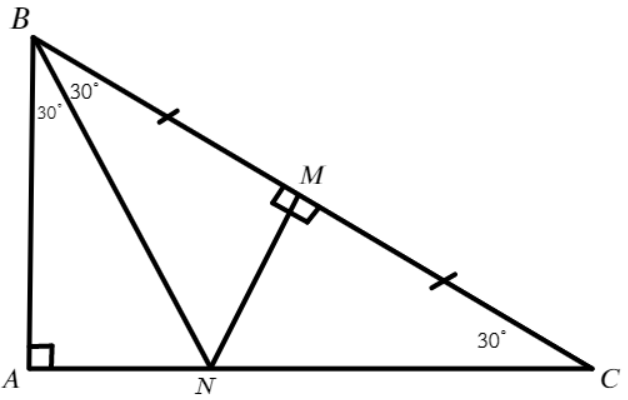
\includegraphics[scale=0.35]{g33.png}}
\end{figure}\\
Пусть $\angle C=30^\circ.$ В треугольнике $NBC$ высота $NM$ совпадает с медианой, значит он равнобедренный и $BN=NC,\ \angle NBC=\angle NCB=30^\circ.$ Тогда $\angle ABN=180^\circ-90^\circ-30^\circ-30^\circ=30^\circ.$ По теореме о катете, лежащем напротив угла в $30^\circ,$ для треугольников $ABN,\ MBN$ и $NMC$ имеем $NC=2NM,\ AN=\frac{1}{2}BN=NM,$ откуда $AC=AN+NC=NM+2NM=3NM,$ ч.т.д.\newpage
\noindent34. \begin{figure}[ht!]
\center{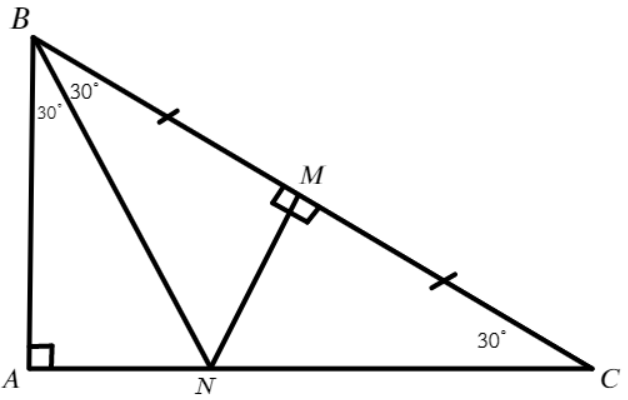
\includegraphics[scale=0.35]{g33.png}}
\end{figure}\\
Пусть $\angle B=60^\circ,$ тогда $\angle C=90^\circ-60^\circ=30^\circ.$ В треугольнике $NBC$ высота $NM$ совпадает с медианой, значит он равнобедренный и $BN=NC,\ \angle NBC=\angle NCB=30^\circ.$ Тогда $\angle ABN=180^\circ-90^\circ-30^\circ-30^\circ=30^\circ.$ По теореме о катете, лежащем напротив угла в $30^\circ,$ для треугольников $ABN,\ MBN$ и $NMC$ имеем $NC=2NM,\ AN=\frac{1}{2}BN=NM,$ откуда $AC=AN+NC=NM+2NM=3NM,$ ч.т.д.\\
